\documentclass[10pt,twocolumn,letterpaper]{article}

\usepackage{cvpr}
\usepackage{times}
\usepackage{epsfig}
\usepackage{graphicx}
\usepackage{amsmath}
\usepackage{amssymb}

% Include other packages here, before hyperref.

% If you comment hyperref and then uncomment it, you should delete
% egpaper.aux before re-running latex.  (Or just hit 'q' on the first latex
% run, let it finish, and you should be clear).
\usepackage[breaklinks=true,bookmarks=false]{hyperref}

\cvprfinalcopy % *** Uncomment this line for the final submission

\def\cvprPaperID{****} % *** Enter the CVPR Paper ID here
\def\httilde{\mbox{\tt\raisebox{-.5ex}{\symbol{126}}}}

% Pages are numbered in submission mode, and unnumbered in camera-ready
%\ifcvprfinal\pagestyle{empty}\fi
%\setcounter{page}{4321}
\DeclareMathOperator*{\argmax}{arg\,max}
\begin{document}

%%%%%%%%% TITLE
\title{Diminished Triad : Consistent Hashing in Redis}

%% TODO: Have to figure out how to add multiple authors
\author{Pallavi Agarwal, Manindra Kumar Moharana, Sanjeev Jagannatha Rao\\
University of California, San Diego\\
%\small PID: A53068263\\
\small p1agarwa,mmoharana,sjrao@ucsd.edu}

% For a paper whose authors are all at the same institution,
% omit the following lines up until the closing ``}''.
% Additional authors and addresses can be added with ``\and'',
% just like the second author.
% To save space, use either the email address or home page, not both


\maketitle
%\thispagestyle{empty}


%%%%%%%%% BODY TEXT
\section{Abstract}
Diminished Triad is a (partial) diminished implementation of chord by the three authors on Redis backends. Redis is an open source, BSD licensed, advanced key-value cache and store.
While Redis offers an extremely fast key value cache, its design suffers from some major drawbacks. Redis does not support consistent hashing, the slaves of a particular master are only aware of the master that they are replicating and unaware of the state of the rest of the system. Redis also does not support automatic migration of keys when a new node joins or readjustment of responsibilities when a node fails. Diminished Triad aims to address these drawbacks of Redis at the cost of an additional layer of indirection and its associated overheads.

\section{Introduction}
"Redis is an open source, BSD licensed, advanced key-value cache and store. It is often referred to as a data structure server since keys can contain strings, hashes, lists, sets, sorted sets and bitmaps"\cite{http://redis.io/topics/introduction} . Twitter, GitHub, Weibo, Pinterest, Snapchat, Craigslist, Digg, StackOverflow and Flickr are some of the well known companies currently using Redis. Redis prides itself on providing very fast performance and several of its design choices have been made with this primary objective. For example, Redis supports asynchronous master slave replication. However, if the master dies before the data is replicated to the slaves, that piece of data is lost. Redis backends are also either only a slave or master and can not be both. A slave replicates a particular master and is unaware of the rest of the system. If a Redis system has r backups, it can support at most r random node failures. If we loose a master and all its slaves we loose all the master's data. Redis contains 16348 key slots. Every key maps to one of these key slots. Redis does not support consistent hashing. When a system is started all the key slots are evenly distributed among the masters.  When a new node joins the system, keys need to be migrated manually to the new node.

In order to achieve its outstanding performance, Redis works with an in-memory dataset. So it offers very high write and read speeds with the limitation that data sets can't be larger than memory. Being an in memory dataset, Redis can work with complicated data structures and supports several of them with very little internal complexity. Redis can persist data by either dumping the dataset to disk every once in a while, or by appending each command to a log. We have adopted the latter approach with our Redis backends as it works like a redo log to migrate data when a new node joins the system. 

In Diminished Triad (DT), we hope to provide a fault tolerant systems using Redis backends that improves on several drawbacks of the existing Redis system described earlier. First,  DT follows a consistent hashing system similar to Chord \cite{Chord}. It hashes every backed and keys to a position on the ring. Second, DT automatically moves keys between nodes every time a node joins or leaves the system. Third, DT system, like chord is completely distributed and no node is more important that the other. 

DT maintains two invariants
\begin{enumerate}
  \item Each node is the master for all the keys that hash between its predecessor and itself.
  \item All the data that a node is responsible for ( keys for which it is the master ) is replicated in the r nodes that follow it on the ring.
\end{enumerate}
Every node is thus a master for some of the keys and is a backup for the r nodes that precede it. Every time a node is added to the system or a node fails and leaves the system, the keys are redistributed amongst all the backends to maintain the two invariants.

The rest of the paper is organized as follows. Section \ref{design} contains the detailed design of Diminished Triad. This section mentions the various components of DT, their individual roles, the APIs used to communicate between these components. Section \ref{implementation} provides the implementation details of DT. Section \ref{evaluation} provides various metrics that measure the performance of Diminished Triad. This section discusses the relative merits and demerits of Diminished Triad over off the shelf Redis.

\section{Design} \label{Design}
We first define several terms that will be helpful in describing the system. 

\begin{enumerate}
  \item User/Client - A user or a client is the customer for the Diminished Triad service. For example, a client requests to set values for some keys, get values etc.
  \item DTServer - All requests like get and set are made by the client to the DTServer. The DTServer then forwards the request to the appropriate backends that are responsible for the key being queried through the DTClient
  \item DTClient - The DTClient is the only channel of communication with the Redis Backend. The DT client transforms the requests received by the DTServer into form understandable by the Redis Backend and queries the appropriate Redis Backend.
  \item DTInstance - DTInstance comprises of the DTServer and a pool of DTClient instances
  \item Redis Backend - This is the off the shelf Redis Server instance that provides all the key value store functionality to Diminished Triad.
  \item DTClientAPI - The user talks only to the DT instance and is unaware of the intricacies of the system. From the user's perspective the DT instances provide a fault tolerant distributed key value store. The DTClientAPI defines all the functions exported by the DTServer to the client. This API makes hides the internal details of DT and makes it look like a fault tolerant key value store to the programmer. A list of all the functions exported DTClientAPI is mentioned later. 
  \item DTServerAPI - The DTInstance, in particular the DTClient talks to the Redis Backends though a set of functions exported by the Redis Backend. This API is completely internal to the DTInstance and the user is completely unaware of the DTServerAPI.
  \item Sentinel - The sentinel is the watchdog for the Redis Backends. It actively monitors if the Redis Backends are working as expected. The Sentinel also notifies through an API when something is wrong with one of the monitored Redis instances.
   \item DTSentinel -  The DTSentinel listens to notifications from the sentinel for any changes like a node leaving the system or joining the system and takes appropriate action in each case to maintain the DT system invariants.
\end{enumerate}

\subsection{System Layout}
Every node runs a Redis Backend and a DTInstance. All DTInstances are identical and none of them are more important than the other. A client can talk to any DTInstance using the DTClientAPI. The DTClient will forward the request to the appropriate Redis Backend using the DTServerAPI. Note that the Redis Backend servicing the client's request may or may not be on the same machine as the DTInstance.
At the moment we have a single Sentinel and DTSentinel instance in our system. We can make our system tolerant to failures of the Sentinel and DTSentinel with minor configuration changes to the Sentinel configuration. The section \ref{fwork} on future work briefly mentions how this can be accomplished. Without loss of generality we will be discussing the system with just one instance of Sentinel and DTSentinel and assume them to be free from failure. Figure \ref{design} shows a typical set for Diminished Triad.

\subsection{DTClientAPI}
Diminished Triad exposes the following functions to the user. This is a subset of the functions exported by the Redis Backend in the DTServerAPI. A complete implementation of Diminished Triad will ideally expose every single function exported by the Redis Backend. We have limited our scope to the functions listed below.
\begin{itemize}
  \item get(key) - gets the value associated with a particular key
  \item set(key,value) - set the value associated with a particular key
  \item getStrlen(key) - get length of a value associated with a particular key
  \item append(key,value) - append a value to the value already associated with a particular key
  \item lPush(key,value) - insert a value in the first position to the list associated with a particular key
  \item lPop(key) - remove and return the first element of the list associated with a particular key
  \item lIndex(key,index) - return the element at a particular index in the list associated with a particular key
  \item lLen(key) - get length of list associated with a particular key
\end{itemize}

\subsection{The Chord Ring, Hashing Keys, Master and the R Backups}
The Chord ring has N positions in it. Every node hosting a DTInstance and a Redis backend is hashed to one of these N positions. Every key is also hashed to one of these N positions. As we move clockwise in the chord ring, we encounter increasing values of hash values until we reach the maximum and then go back to 0. Every backend is the master for the all the keys that hash to its position in the ring through the hash positions up to but not including its  predecessor in the ring. The predecessor of a backend is defined as the first live backend that is encountered as we move anti clockwise in the chord ring. Similarly the successor is the first live backend that is encountered as we move clockwise in the chord ring. The r backends that immediately succeed the master serve as the r backups of that particular master.



\section{Implementation} \label{implementation}
system implementation here

\section{Evaluation} \label{evaluation}
system design here

\section{Dataset}
The CIFAR-10 dataset \cite{krizhevsky2009learning} consists of 60000 32x32 images belonging to 10 classes with 6000 images per class.	The training set consists of 50000 images and the test set consists of 10000 images. The classes are mutually exclusive with almost no overlap between images.

\begin{figure}[hbt]
  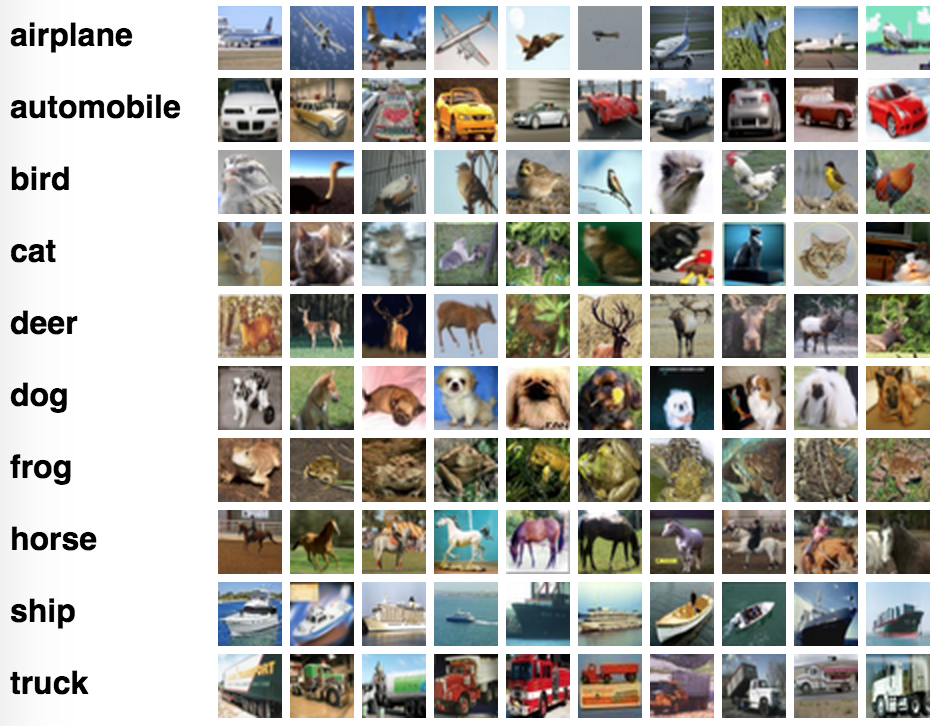
\includegraphics[scale=0.50]{cifar-dataset}
  \caption{10 random images from 10 classes of the CIFAR-10 dataset}
\end{figure}

\section{Why CNN?}
Traditional neural networks (NNs) receive some input and transform it through a series of hidden layers. Every layer consists of some neurons which are fully connected to all neurons of the previous layer. The neurons in a layer function independently without sharing connections.

In CIFAR-10, images are 32x32x3 (3 color channels), so a regular neural network would have 32*32*3 = 3072 weights. If we need multiple such layers, the number of weights could increase very quickly to an unmanageable degree. Therefore, this full connectivity is undesired and training too many parameters can lead to overfitting. CNNs have a special architecture to take advantage of the 2D shape of images. The layers in a CNN are arranged in 3 dimensions - width, height, depth. The neurons in a layer are connected to a small region of the layer before it, instead of a fully connected manner. Therefore they have lesser parameters than a fully connected network with same number of hidden units.

\section{Recent Work with CNNs}
We will now take a look at some of the existing work in image classification using CNNs. CNNs were first introduced by Kunihiko Fukushima in 1980 \cite{fukushima1980neocognitron}. LeCun et. al. \cite{lecun1998gradient} improved the design and proposed LeNet-5, a 7 layer CNN for classifying handwritten digits in the MNIST dataset. Krizhevsky et. al. \cite{krizhevsky2012imagenet} broke new grounds in CNNs by achieving state of the art error rate on ImageNet LSVRC-2012 contest using a 8 layer deep CNN. Hinton et. al. \cite{hinton2012improving} proposed an enhancement for CNNs using a random dropout layer that greatly reduced overfitting.
	The state of the art accuracy of 91.78\% in CIFAR-10 was achieved by Lee et. al. \cite{lee2014deeply} using their Deeply Supervised Net architecture which uses an additional companion objective function for the hidden layers, that is minimized along with the global loss. The network in network model by Lin et. al. \cite{DBLP:journals/corr/LinCY13} achieved an accuracy of 91.2\%.


\section{Layers in a CNN}
A CNN consists of a number of convolution and subsampling(pooling) layers, followed by a fully connected layer as output. 
\subsection{Convolution Layer}
The convolution layer can be interpreted as a 3D volume containing neurons along its depth \cite{cnnref}. Its parameters consist of a set of learnable filters which extend along the depth. In the forward process, each filter is convolved with a particular patch of the image along the depth. Intuitively, the network will learn filters that activate when a particular feature is observed in that part of the image.

\subsection{Pooling Layer}
Pooling layers are usually added between convolution layers in a CNN. This layer is used to reduce the size of the representation so that the computation and number of parameters in the network are reduced. It also helps prevent overfitting. This layer operates on every depth slice of the input layer and reduces it spatially using a pooling function. Common pooling functions are max  pooling, average pooling and L-2 norm pooling. For example, if the kernel size is 2x2, it reduces 4 inputs to 1 output by applying the pooling function on the inputs.

\subsection{Fully connected Layer}
The neurons of this layer are fully connected to all activations of the previous layer.

\subsection{Loss Layer}
This layer computes the loss with respect to a target and assigns the cost needed to mininmize the loss. The loss is computed in the forward pass and the the gradient w.r.t loss is computed in the backward pass. Common loss functions include softmax loss, euclidean distance loss and hinge loss.

\subsection{ReLU Layer}
The rectified linear unit is a recently introduced layer that has gained popularity. This layer computes the function $f(x) = max(x,0)$. It's basically a zero thresholding layer. It has been shown to significantly decrease the training time (by a factor of 6 as reported by Krizhevsky et al.).

\subsection{Dropout Layer}
The dropout layer is a recent important invention in neural networks by Hinton et. al. \cite{hinton2012improving}. It addresses a fundamental problem in machine learning - overfitting. It accomplishes this by setting certain activations to zero (dropping out) during the training phase. For each training example, a different set of random units is selected to drop. The number of activations to be dropped is controlled by a dropout ratio parameter.

% Existing Methods, Describe dataset, Describe each of the 3 algo, Exp setup,
% Results, Conclusion
%-------------------------------------------------------------------------



\section{Caffe}
Caffe is an open source deep learning framework developed by the Berkeley Vision and Learning Center. It's implemented in C++/Cuda and provides command line, python and Matlab interfaces. Caffe is built with speed in mind, and provides seamless switching between CPU and GPU. Another advantage of Caffe is that models can be written entirely using schemas, without writing any code. For this project, I'll be making use of Caffe to train multiple CNNs for CIFAR-10 classification.

\section{Experiments}

I created and trained multiple Caffe models and evaluated their performance on the CIFAR-10 dataset. For maintaining consistency, I trained each network for 20K epochs using SGD and compared their performance on the test set. I used a learning rate of 0.001 for the first 10K epochs and 0.00001 for the next 10K epochs. I used the softmax loss function in the last loss layer.

The first network I tried is a 4 layer network consisting of 2 pairs of convolution and max pooling layers. It's architecture is described in table \ref{net1}.

\begin{table}[h]

\begin{tabular}{|l|l|l|}
\hline
Layer Type & Parameters                     & Outputs \\ \hline
CONV       & Kernel: 5x5, Pad: 2, Stride: 1 & 32      \\ \hline
MAX POOL   & Kernel: 3x3, Stride: 1         &         \\ \hline
CONV       & Kernel: 5x5, Pad: 1, Stride: 1 & 32      \\ \hline
MAX POOL   & Kernel: 3x3, Stride: 1         &         \\ \hline
FC         &                                & 10      \\ \hline
\end{tabular}
\label{net1}
\caption{CNN 1}
\end{table}

This network had an accuracy of 72.91\% after 20K epochs. I had tried different kernel sizes of 3x3, 5x5 and 7x7, and zero padding values of 1,2 and 3. Kernel size of 5x5 for convolution layers and 3x3 for max pooling layers gave me the best accuracy.

I tried adding ReLU layers at the end of each max pooling layers in the above network. This improved accuracy by a decent margin - 75.81\%. Thus, proving that ReLU units indeed decrease training time, as the network was able to achieve higher accuracy with same number of epochs.

After this, I tried the 6 layer network by Krizhevsky and also added ReLU layers, as described in table 2.

\begin{table}[h]
\begin{tabular}{|l|l|l|}
\hline
Layer Type & Parameters                     & Outputs \\ \hline
CONV       & Kernel: 5x5, Pad: 2, Stride: 1 & 32 + ReLU     \\ \hline
MAX POOL   & Kernel: 3x3, Stride: 1         &         \\ \hline
CONV       & Kernel: 5x5, Pad: 1, Stride: 1 & 32 + ReLU      \\ \hline
AVG POOL   & Kernel: 3x3, Stride: 1         &         \\ \hline
CONV       & Kernel: 5x5, Pad: 1, Stride: 1 & 64 + ReLU     \\ \hline
AVG POOL   & Kernel: 3x3, Stride: 2         &         \\ \hline
FC         &                                & 10      \\ \hline
\end{tabular}
\label{net2}
\caption{CNN 2}
\end{table}

This layer makes use of 1 max pooling layer and 2 average pooling layers. It has an accuracy of 77.39\%. I tried adding dropout layers to the above network to try to improve accuracy. I modified the network to the following:

\begin{table}[h]
\begin{tabular}{|l|l|l|}
\hline
Layer Type & Parameters                     & Outputs \\ \hline
CONV       & Kernel: 5x5, Pad: 2, Stride: 1 & 32 + ReLU     \\ \hline
MAX POOL   & Kernel: 3x3, Stride: 1         &         \\ \hline
CONV       & Kernel: 5x5, Pad: 1, Stride: 1 & 32 + ReLU      \\ \hline
AVG POOL   & Kernel: 3x3, Stride: 1         &         \\ \hline
DROPOUT   & Dropout ratio: 0.25         &         \\ \hline
CONV       & Kernel: 5x5, Pad: 1, Stride: 1 & 64 + ReLU     \\ \hline
AVG POOL   & Kernel: 3x3, Stride: 2         &         \\ \hline
DROPOUT   & Dropout ratio: 0.25         &         \\ \hline
FC         &                                & 10      \\ \hline
\end{tabular}
\label{net3}
\caption{CNN 3}
\end{table}

Adding dropout further improved the accuracy to 79.57\%. I tried other dropout ratios like 0.10, 0.20 and 0.50. 0.25 dropout gave the best performance. The filters of the three convolution layers are shown in figures 2, 3, 4.


\begin{figure}[hbt]

  \centering
  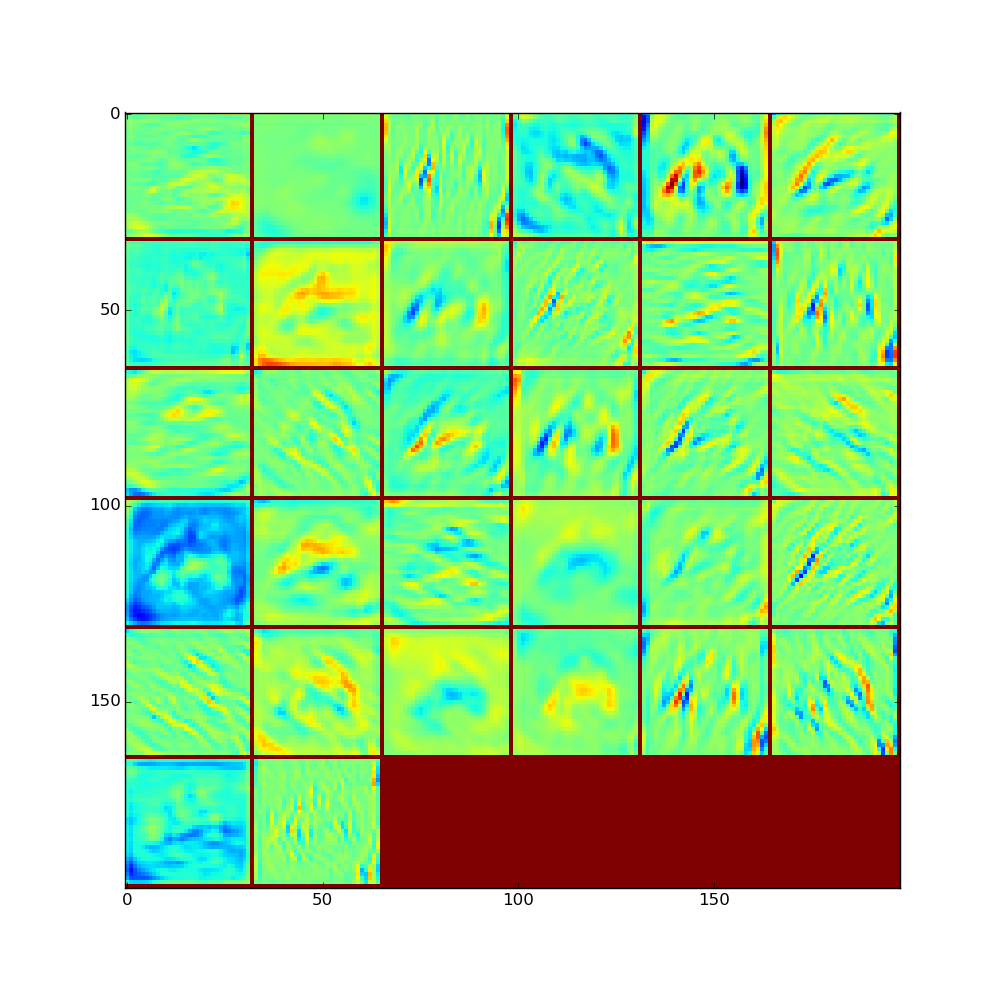
\includegraphics[scale=0.32]{d1}
  	\label{l1}
  \caption{Filters in first convolution layer for CNN in table 3}
\end{figure}
\begin{figure}[hbt]

  \centering
  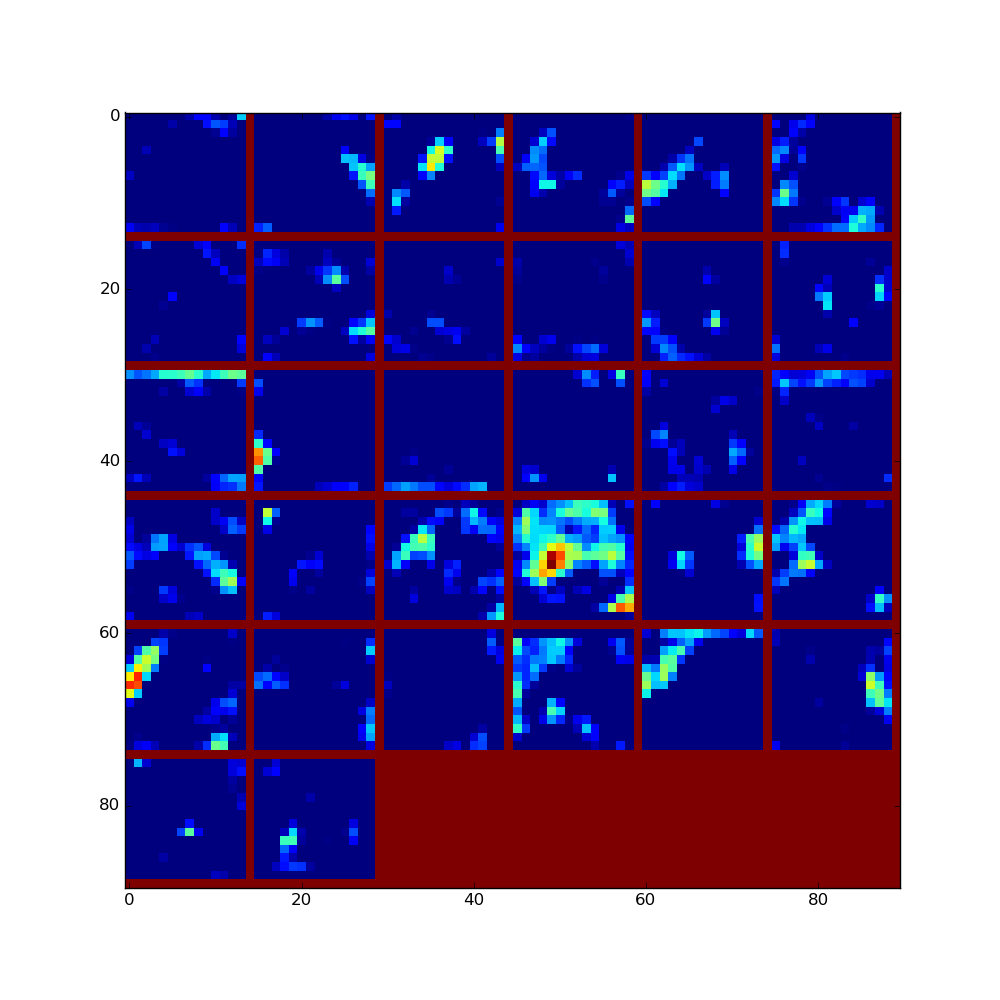
\includegraphics[scale=0.32]{d2.png}
  \label{l2}
  \caption{Filters in second convolution layer for CNN in table 3}
\end{figure}
\begin{figure}[hbt]

  \centering
  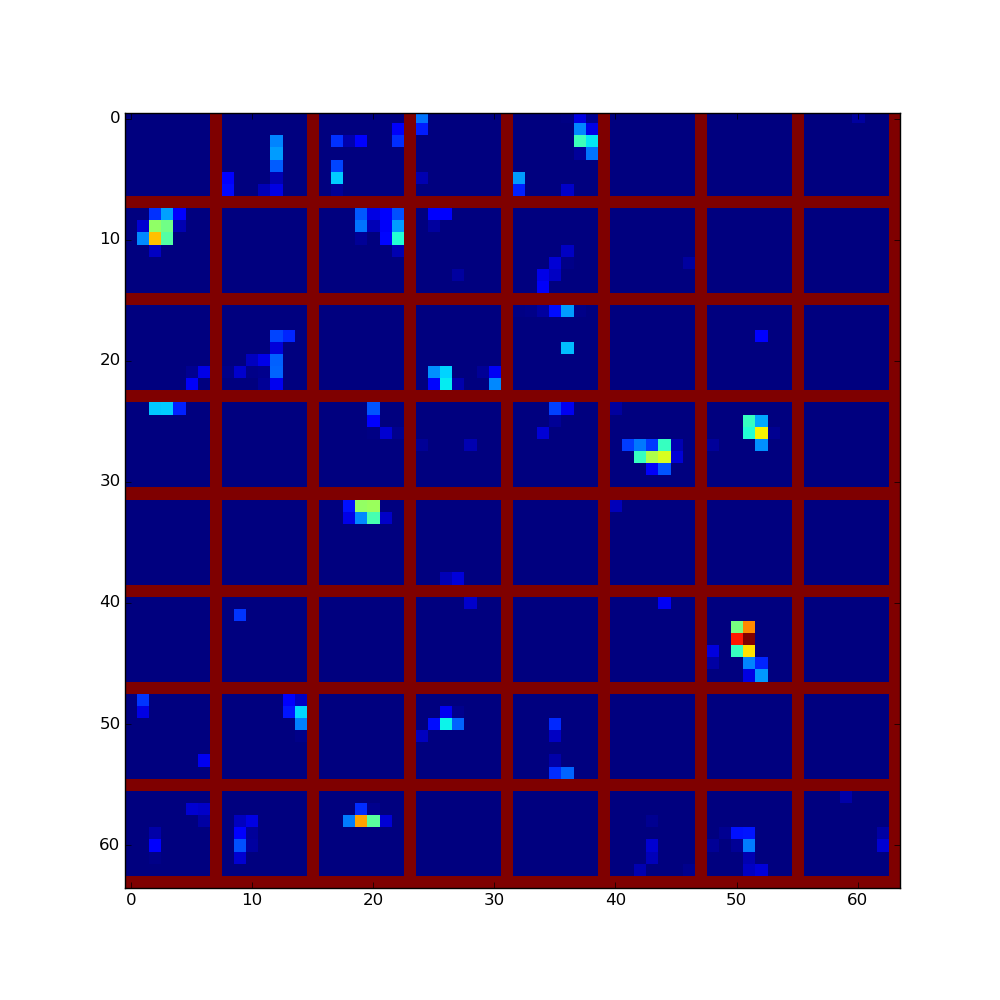
\includegraphics[scale=0.32]{d3.png}
  \label{l3}
  \caption{Filters in second convolution layer for CNN in table 3}
\end{figure}

As one can see from the filter images, the earlier stage filters activate on large image patches whereas deeper filters learn to activate on small/specific locations in the image. The intuition is that with successive layers, filters learn to focus on specific small features within an image.

Finally I compared my results to the reference CIFAR-10 classifier included in Caffe. This net makes use of 2 normalization layers in addition to the Krizhevsky network. This net achieves an accuracy of 77.48\%.

\section{Results}

I trained 4 different networks in Caffe, successively iterating and improving the accuracy. The results are summarised in table 4. My final 6 layer model using relu and dropout was able to beat the reference model included in Caffe by a small margin. I observed that adding higher number layers improves performance at the cost of training time. But adding too many layers can also have the potential downside of overfitting to the training data and performing badly on the unseen test data. Dropout can help mitigate this to a certain extent.

\begin{table}[h]
\begin{tabular}{|l|l|}
\hline
Model & Accuracy \\ \hline
4 layer & 72.91\%    \\ \hline
4 layer $+$ ReLU & 72.91\%    \\ \hline
6 layer $+$ ReLU, Avg Pooling & 77.39\%    \\ \hline
6 layer $+$ Dropout, ReLU, Avg Pooling & \textbf{79.57\%}    \\ \hline
Caffe Model $+$ ReLU, Avg Pooling, Normalization & 77.48\%    \\ \hline
\end{tabular}
\label{result}
\caption{Results}
\end{table}

\section{Conclusion and Future Scope}

In this project, I got to learn how to prototype models using the powerful Caffe framework and achieved decent results on the CIFAR-10 dataset. If I had more time, I would have tried to the train the models for much higher number of epochs. The state of the art models are trained for 150000+ epochs. Ensemble models are also known to improve performance. Data augmentation (mirroring, rotations, affine transformations) is another technique used to increase the size of training data and thus improve performance.

In the future, I would like to train deeper networks for higher number of epochs and also explore how to use ensemble models and data augmentation techniques for improving performance.

\section{Acknowledgements}

I would like to thank Professor Zhuowen Tu and 2Lab for providing access to their lab server with which I was able to use GPUs to speed up the training in Caffe.
 

{\small
\bibliographystyle{ieee}
\bibliography{egbib}
}

\end{document}
